\documentclass{file/TA-ITS}
%Ridho Nur Rohman Wijaya

\makeatletter
\def\cleardoublepage{\clearpage%
	\if@twoside
	\ifodd\c@page\else
	\vspace*{\fill}
	\hfill
	\begin{center}
		\emph{ }
	\end{center}
	\vspace{\fill}
	\thispagestyle{empty}
	\newpage
	\if@twocolumn\hbox{}\newpage\fi
	\fi
	\fi
}
\makeatother
\newtheorem{defn}{Definisi}[section]
\newtheorem{teo}[defn]{Teorema}
\newtheorem{thm}{Teorema}[section]
\newtheorem{lemma}[defn]{Lemma}
\newtheorem{lemmas}[thm]{Lemma}
\newtheorem{cor}[defn]{Akibat}
\theoremstyle{definition}
\newtheorem{con}[defn]{Contoh}
\theoremstyle{definition}
\theoremstyle{plain}
\newtheorem{prop}[defn]{Proposisi}
\renewcommand{\proofname}{Bukti}
\renewcommand{\thethm}{\arabic{chapter}.\arabic{thm}}

\newcommand{\norm}[1]{\left\|#1\right\|} % Fungsi norm (||x||)

\newcommand\firstPar{0.75cm} % Indentasi 0.75cm pada tiap paragraf (manual untuk hspace)
\setlength{\parindent}{0.75cm} % Indentasi 0.75cm pada tiap paragraf

\usepackage{fancyhdr}
\pagestyle{fancy}
\renewcommand{\headrulewidth}{0pt}
\fancyhf{}
\usepackage{ifthen}
\fancyfoot[R]{\ifthenelse{\isodd{\value{page}}}{\thepage}{}}
\fancyfoot[L]{\ifthenelse{\isodd{\value{page}}}{}{\thepage}}

\usepackage[labelsep=quad]{caption}
\captionsetup[table]{skip=5pt}

\usepackage{multirow}
\usepackage{longtable}
\usepackage{physics}
\usepackage{ragged2e} 
\usepackage[mathscr]{eucal}

% Pengaturan tabel
\usepackage{multicol,multirow}
\newcommand{\blue}{\cellcolor{blue!100}}
\newcommand{\red}{\cellcolor{red!75}}
\newcommand{\yellow}{\cellcolor{yellow!75}}
\newcommand{\gray}{\cellcolor{gray!75}}
\newcommand{\cyan}{\cellcolor{cyan!100}}
\usepackage{longtable} % Pembuatan tabel
\usepackage[table,xcdraw]{xcolor} % Pewarnaan tabel
% Inisiasi lebar kolom tabel
\newcolumntype{L}[1]{>{\raggedright\let\newline\\\arraybackslash\hspace{0pt}}m{#1}}
\newcolumntype{C}[1]{>{\centering\let\newline\\\arraybackslash\hspace{0pt}}m{#1}}
\newcolumntype{R}[1]{>{\raggedleft\let\newline\\\arraybackslash\hspace{0pt}}m{#1}}

%%% Pewarnaan code
\usepackage{xcolor}
\usepackage{color}
\usepackage{listings}

\definecolor{codegreen}{rgb}{0,0.6,0}
\definecolor{codeblack}{rgb}{0,0,0}
\definecolor{codepurple}{rgb}{0.58,0,0.82}
\definecolor{backcolour}{rgb}{0.95,0.95,0.92}

\lstdefinestyle{mystyle}{
    commentstyle=\color{codegreen},
    keywordstyle=\color{magenta},
    numberstyle=\tiny\color{codeblack},
    stringstyle=\color{codepurple},
    basicstyle=\ttfamily\footnotesize,
    breakatwhitespace=false,         
    breaklines=true,                 
    captionpos=b,                    
    keepspaces=true,                 
    numbers=left,                    
    numbersep=5pt,                  
    showspaces=false,                
    showstringspaces=false,
    showtabs=false,                  
    tabsize=2
}
%%% Pewarnaan code

\hypersetup{ % Merubah warna link
    colorlinks,
    linkcolor={black},
    citecolor={black},
    urlcolor={black}
}

% \tolerance=1
% \emergencystretch = \maxdimen
% \hyphenpenalty=10000
% \hbadness=1000

\begin{document}

% input data
\Judul{Optimisasi Jadwal Jaringan Bus di Terminal Purabaya Menggunakan Aljabar Max-Plus}

\JudulEng{Optimization of Bus Network Scheduling at Purabaya Terminal Using Max-Plus Algebra}

\Nama{Teosofi Hidayah Agung}

\NamaKecil{Teosofi Hidayah Agung}

\NRP{5002221132}

\Departemen{Matematika}

\Department{Mathematics}

\BidangStudi{Aljabar dan Analisis}

\Bulan{November} % Masuk lembar pengesahan

\Tahun{2024}

\TanggalDisetujui{22 November 2024} % Masuk lembar orisinilitas

\Fakultas{Sains dan Analitika Data}

\SingkatanFakultas{FSAD}

\Faculty{Scientics}

\SingkatanFakultasEng{SCIENTICS}

\Pembimbing{Pembimbing 1}
          {} % Isi {} untuk pembimbing 2
		   

\NIPPembimbing{NIP}
{} % Isi {} untuk pembimbing 2
              
              
\Penguji{Penguji 1}
        {Penguji 2}
        {Penguji 3}

\NIPPenguji{NIP Penguji 1}
           {NIP Penguji 2}
           {NIP Penguji 3}
\Kadep{Nama Kadept}

\NIPKadep{NIP Pak Kadept}
%\Cover
\BagianAwal
\LembarJudul
\TitlePage
%\LembarPengesahan
%\LembarOrisinalitas
\LembarPengesahanProposal
\LembarAbstrak
\LembarAbstract

%%%%%%%%%%%%%%%%%%%%%%%%  Abstrak  %%%%%%%%%%%%%%%5%%%%%%%%%%
%\input{Inti/abstrak}

%%%%%%%%%%%%%%%%%%%%%%%%  Abstrak  %%%%%%%%%%%%%%%5%%%%%%%%%%


%%%%%%%%%%%%%%%%%%%%%%%%  Daftar  %%%%%%%%%%%%%%%5%%%%%%%%%%

\DaftarIsi\raggedbottom

\DaftarGambar
%%%%%%%%%%%%%%%%%%%%%%%%  Daftar  %%%%%%%%%%%%%%%5%%%%%%%%%%

\DaftarTabel
%%%%%%%%%%%%%%%%%%%%%%%%  Daftar  %%%%%%%%%%%%%%%5%%%%%%%%%%

\DaftarSimbol
%%%%%%%%%%%%%%%%%%%%%%%%  Daftar  %%%%%%%%%%%%%%%5%%%%%%%%%%

\BagianInti

%%%%%%%%%%%%%%%%%%%%%%%%  Bab I-III  %%%%%%%%%%%%%%%5%%%%%%%%%%

\pagebreak
\chapter{PENDAHULUAN}
\section{Latar Belakang}
Perkembangan teknologi militer di era modern merupakan faktor penting untuk menjaga keamanan negara. Salah satu bentuk perkembangan teknologi pertahanan adalah sistem persenjataan jarak jauh yang mampu menghancurkan target dengan akurasi tinggi. 

\section{Rumusan Masalah}
Rumusan masalah yang diangkat pada penelitian ini adalah sebagai berikut:
\begin{enumerate} 
    \item 
    \item 
\end{enumerate}

\section{Batasan Masalah}
Batasan masalah dalam penelitian ini adalah sebagai berikut :
\begin{enumerate}
    \item  
    \item 
\end{enumerate}
 
\section{Tujuan}
\begin{enumerate}
    \item 
    \item 
\end{enumerate}

\section{Manfaat}
\begin{enumerate}
 \item 
 \item  
 \item 
\end{enumerate}

\pagebreak
\chapter{TINJAUAN PUSTAKA}
\section{Hasil Penelitian Terdahulu}

\begin{table}[h]
  \centering
  \begin{tabular}{|p{3cm}|p{1.2cm}|p{3cm}|p{6cm}|}
    \hline
    \textbf{Penulis}                                                                   & \textbf{Tahun} & \textbf{Judul} & \textbf{Rangkuman}                             \\
    \hline
    Muhammad Zulfikar Zufar                                                            & 2023           & Kontruksi Grup
    Latin Square pada Aljabar Max-Plus                                                 &                                                                                  \\
    \hline

    Muhammad Syifa'ul Mufid and Subiono                                                &
    2014                                                                               &
    Eigenvalues and eigenvectors of Latin Squares In Max-plus Algebra                  &
    Diselesaikan Permasalahan Eigen dari \textit{latin square} pada Aljabar Max-plus dengan Memperhatikan Permutasi dari Angka-angka pada \textit{latin square} Tersebut. \\
    \hline

    Kasie G Farlow                                                                     &
    2009                                                                               &
    Max-Plus Algebra                                                                   &
    Dibahas Mengenai Beberapa Hal Terkait Aljabar Max-plus, dan Salahsatu Hal Menarik yang Dibahas pada Paper ini adalah Aljabar Linear pada Aljabar Max-plus.            \\
    \hline

    Fazal Abbas and Mubasher Umer and Umar Hayat and Ikram Ullah                       &
    2022                                                                               &
    Trivial and Nontrivial eigenvectors for \textit{latin squares} in Max-Plus Algebra &
    Mengkaji Permasalahan Eigen pada \textit{Non-Symmetric} Latin Square pada Aljabar Max-plus.                                                                           \\
    \hline
  \end{tabular}
  \caption{Ringkasan Literatur terkait Max-Plus Algebra dan Latin Squares}
\end{table}



\pagebreak
\chapter{METODOLOGI}

Pada bab ini akan dijelaskan langkah-langkah pelaksanaan penelitian tugas akhir yang dilengkapi dengan alur proses serta jadwal kegiatan yang disusun selama penelitian.
% \section{Studi Literatur}
% Pada tahap ini dilakukan pengumpulan referensi yang relevan dengan penelitian tugas akhir ini. Sumber referensi yang digunakan adalah buku, tugas akhir, tesis, paper, serta artikel yang mendukung topik penelitian. Referensi yang terkait dengan penelitian ini adalah mengenai kendali rudal menggunakan metode NMPC dengan pendekatan fungsi laguerre.

\section{Pengkajian Model Matematika Rudal}

\section{Pendiskritan Model}

\section{Pembentukan Kendali Rudal Menggunakan Laguerre-NMPC}

\section{Simulasi dan Analisis Hasil Simulasi}

\section{Penarikan Kesimpulan dan Saran}

\section{Penulisan Laporan Tugas Akhir}

\begin{figure}[htbp]
    \centering
    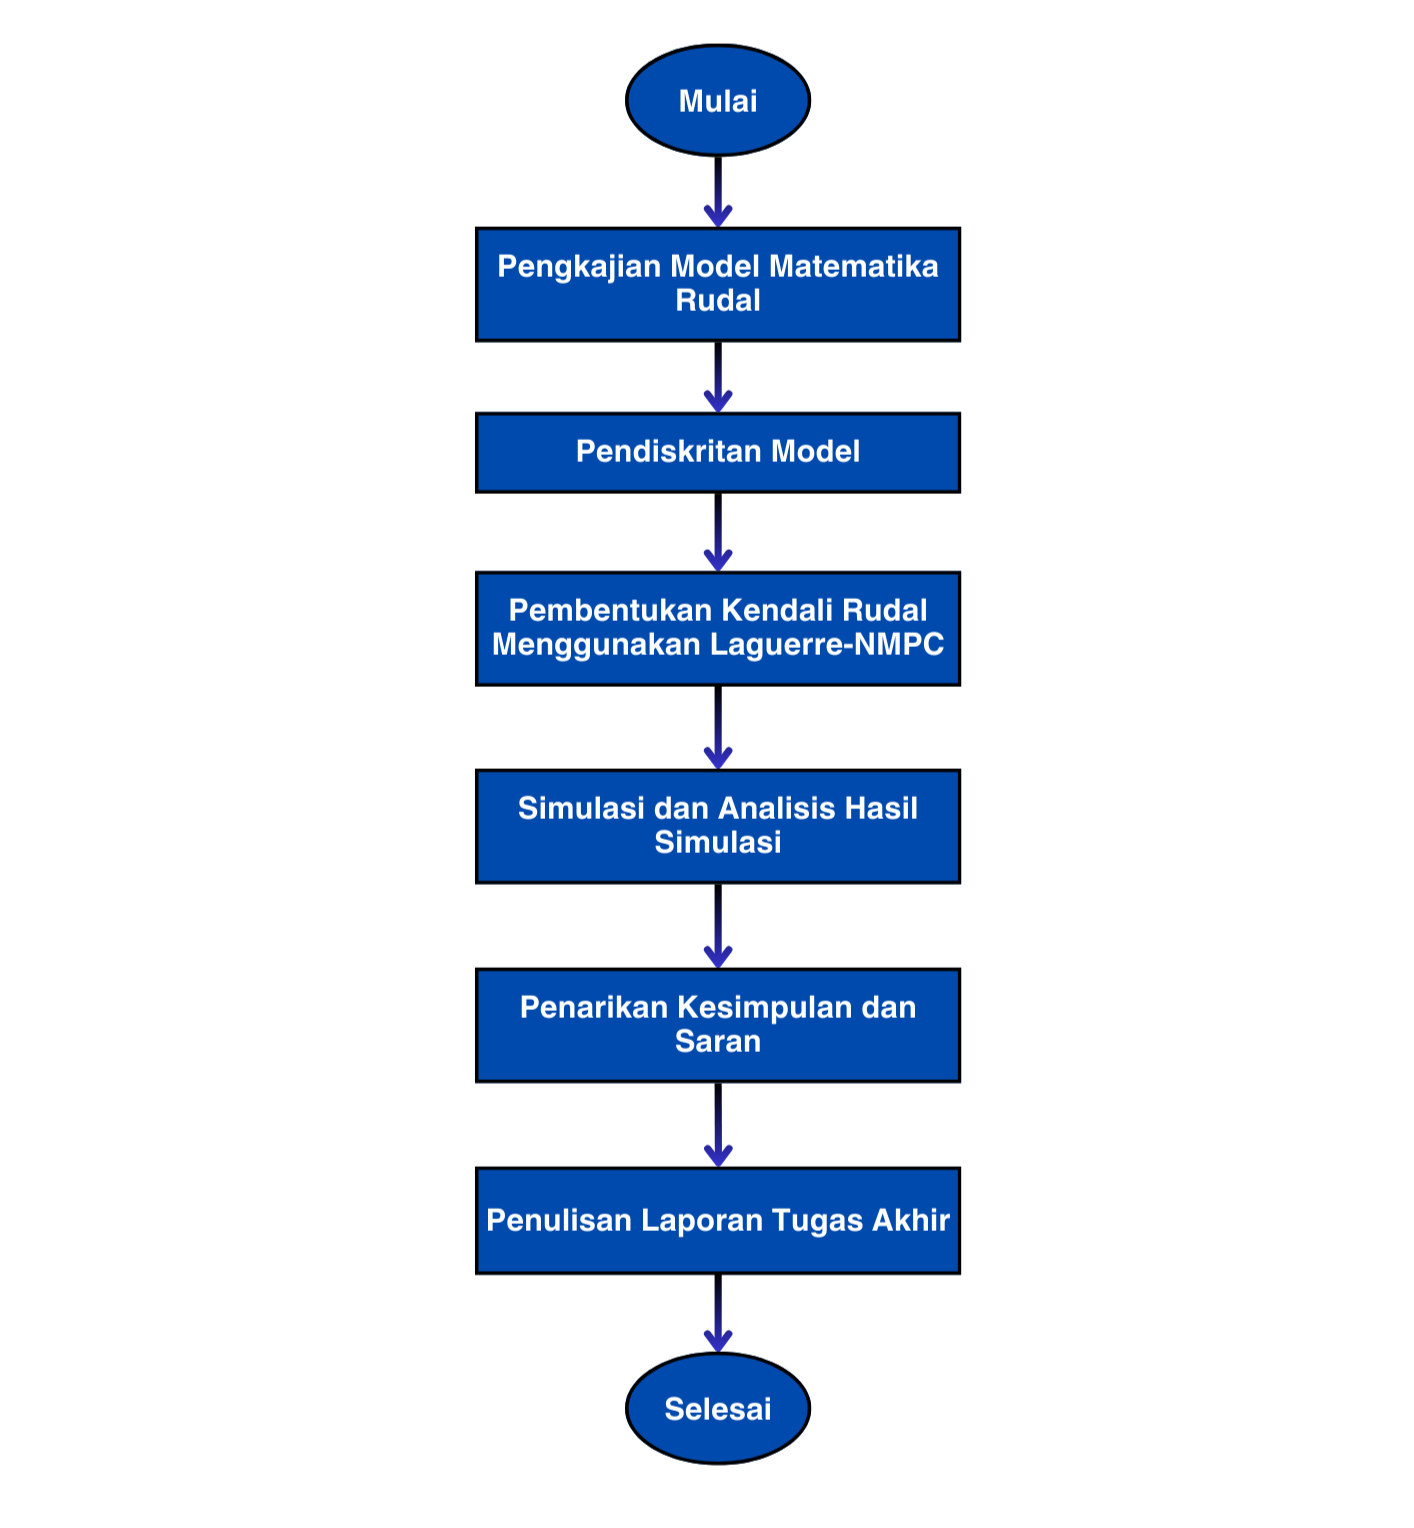
\includegraphics[width=\linewidth]{foto/Diagram Alir Penelitian Blue.png}
    \caption{Diagram Alir Penelitian}
    \label{fig:diagram penelitian}
\end{figure}

\pagebreak
\chapter*{JADWAL PENELITIAN}
Berikut jadwal pelaksanaan tahap-tahap penelitian tugas akhir yang akan dilakukan selama 3 bulan sesuai dengan metode penelitian. \vspace{0.5cm}
\begin{table}[htbp]
\centering
\caption{Jadwal Pelaksanaan Penelitian Tugas Akhir}
\renewcommand{\arraystretch}{1.5}
\begin{tabular}{|C{0.6cm}|L{6.5cm}|C{0.25cm}|C{0.25cm}|C{0.25cm}|C{0.25cm}|C{0.25cm}|C{0.25cm}|C{0.25cm}|C{0.25cm}|C{0.25cm}|C{0.25cm}|C{0.25cm}|C{0.25cm}|}	\hline
	&&\multicolumn{12}{c|}{\textbf{BULAN}}\\\cline{3-14}
	\multicolumn{1}{|c|}{\textbf{NO}}&\multicolumn{1}{c|}{\textbf{NAMA KEGIATAN}}&\multicolumn{4}{c|}{1}&\multicolumn{4}{c|}{2}&\multicolumn{4}{c|}{3}\\\cline{3-14}
	&&1&2&3&4&1&2&3&4&1&2&3&4\\\cline{1-14}
	1&Pengkajian model matematika rudal &\cellcolor{blue!}&\cellcolor{blue!}&&&&&&&&&&\\\hline
	2&Pendiskritan model&&\cellcolor{blue!}&\cellcolor{blue!}&&&&&&&&&\\\hline
	3&Pembentukan kendali rudal menggunakan Laguerre-NMPC &&&\cellcolor{blue!}&\cellcolor{blue!}&&&&&&&&\\\hline
	4&Pembuatan program menggunakan software MATLAB R2024b &&&&\cellcolor{blue!}&\cellcolor{blue!}&\cellcolor{blue!}&\cellcolor{blue!}&&&&&\\\hline
	5&Simulasi dan analisis hasil simulasi&&&&&&&\cellcolor{blue!}&\cellcolor{blue!}&\cellcolor{blue!}&&&\\\hline
	6&Penarikan kesimpulan dan saran&&&&&&&&&\cellcolor{blue!}&\cellcolor{blue!}&&\\\hline
	7&Penulisan laporan tugas akhir&&&&&&&&&&\cellcolor{blue!}&\cellcolor{blue!}&\cellcolor{blue!}\\\hline
\end{tabular}
\end{table}

%\pagebreak
\chapter{Hasil dan Pembahasan}

\section{Analisis Model Matematika Rudal}
Pada penelitian tugas akhir ini, jenis rudal yang digunakan adalah rudal balistik RX-200 TC (BRIN). Model matematika yang digunakan terdiri dari model kinematika rudal dengan 3 derajat kebebasan dan model dinamika rudal dengan 3 derajat kebebasan. Nilai parameter rudal balistik RX-200 TC (BRIN) terdapat pada \ref{tab: parameter rudal}.

% \begin{table}[htbp]
%     \setlength{\tabcolsep}{10pt}
%     \renewcommand{\arraystretch}{1.8}
%     \centering
%     \caption{Nilai Parameter pada Rudal Balistik RX-200 TC (BRIN)}
%     \begin{tabular}{|c| c| c| c| c| c|c| c| c|}
%     \hline
%         \textbf{No} & \textbf{Notasi} & \textbf{Nilai} & \textbf{No} & \textbf{Notasi} & \textbf{Nilai} & \textbf{No} & \textbf{Notasi} & \textbf{Nilai} \\ \hline 
%         1 & $\alpha$ &  & 17 & $C_X$ &  & 33 & $M$ &  \\ \hline
%         2 & $\beta$ &  & 18 & $C_{X_{\dot{\alpha}}}$ &  & 34 & $\dot{M}$ &  \\ \hline
%         3 & $C_{l_{\beta}}$ &  & 19 & $C_{X_{q}}$ &  & 35 & $g$ &  \\ \hline
%         4 & $C_{l_{p}}$ &  & 20 & $C_{X_{\delta_a}}$ &  & 36 & $\hat{q}$ &  \\ \hline
%         5 & $C_{l_{r}}$ &  & 21 & $C_{X_{\delta_e}}$ &  & 37 & $c$ &  \\ \hline
%         6 & $C_{l_{\delta_a}}$ &  & 22 & $C_{X_{\delta_r}}$ &  & 38 & $S$ &  \\ \hline
%         7 & $C_{l_{\delta_r}}$ &  & 23 & $C_{Y_{\beta}}$ &  & 39 & $d$ &  \\ \hline
%         8 & $C_{m}$ &  & 24 & $C_{Y_{p}}$ &  & 40 & $I_x$ &  \\ \hline
%         9 & $C_{m_{{\dot{\alpha}}}}$ &  & 25 & $C_{Y_{r}}$ &  & 41 & $I_y$ &  \\ \hline
%         10 & $C_{m_{q}}$ &  & 26 & $C_{Y_{\delta_r}}$ &  & 42 & $I_z$ &  \\ \hline
%         11 & $C_{m_{\delta_e}}$ &  & 27 & $C_{Y_{\delta_a}}$ &  & 43 & $\dot{I_x}$ &  \\ \hline
%         12 & $C_{n_{\beta}}$ &  & 28 & $C_{Z}$ &  & 44 & $\dot{I_y}$ &  \\ \hline
%         13 & $C_{n_{p}}$ &  & 29 & $C_{Z_{\dot{\alpha}}}$ &  & 45 & $\dot{I_z}$ &  \\ \hline 
%         14 & $C_{n_r}$ &  & 30 & $C_{Z_{q}}$ &  & 46 & $m$ &  \\ \hline 
%         15 & $C_{n_{\delta_a}}$ &  & 31 & $C_{Z_{\delta_e}}$ &  & 47 & $x_e$ & \\ \hline 
%         16 & $C_{n_{\delta_r}}$ &  & 32 & $T$ &  &  &  &  \\ \hline
%     \end{tabular}
%     \label{tab: parameter rudal}
% \end{table}

\begin{table}[htbp]
 \setlength{\tabcolsep}{10pt}
 %\renewcommand{\arraystretch}{1.5}
    \centering
    \caption{Nilai Parameter Rudal Balistik RX-200 TC (BRIN)}
    \begin{tabular}{|c|l|c|}
    \hline 
        \textbf{Notasi} & \multicolumn{1}{c|}{\textbf{Parameter}}  & \textbf{Nilai} \\
        \hline
        $m$ & Massa roket & 197.03 $kg$\\
        \hline
        $\dot{m}$ & Perubahan massa roket & 8.05 $kg/s$ \\
        \hline
        $T$ & Gaya dorong roket & \dots  \\
        \hline
        $g$ & gravitasi bumi & 9.806 $m/s^2$ \\
        \hline
        $\hat{q}$ & Tekanan dinamik & 63460 $N/m^2$ \\
        \hline
        $c$ & Diameter roket & 0.203 $m$ \\
        \hline
        $S$ & Luas penampang badan roket & 0.0324 $m^2$ \\
        \hline
        $\dot{\alpha}$ & \textit{Rate of change of Angle of attack} & -0.00407 \\
        \hline
        % $\beta$ & \textit{Side slip angle}  &  \\
        % \hline
        $x_e$ & pusat aliran massa & 1247 \\
        \hline 
        $d$ & Perubahan titik pusat massa & \dots \\
        \hline
        $I_x$ & Momen Inersia $x$ & 1.252 $kg\,m^2$ \\
        \hline
        $I_y$ & Momen Inersia $y$ & 188.470 $kg\,m^2$ \\
        \hline
        $I_z$ & Momen Inersia $z$ & 188.472  $kg\,m^2$ \\
        \hline
        $\dot{I_x}$ & Perubahan Momen Inersia $x$ & 0.036  $kg\,m^2/s$ \\
        \hline
        $\dot{I_y}$ & Perubahan Momen Inersia $y$ & 4.612  $kg\,m^2/s$ \\
        \hline
        $\dot{I_z}$ & Perubahan Momen Inersia $z$ & 4.612 $kg\,m^2/s$ \\
        \hline
    \end{tabular}
    \label{tab: parameter rudal}
\end{table}


\subsection{Model Matematika Kinematika Rudal}

Model matematika kinematika rudal 3 derajat kebabasan terdiri dari kinematika translasi dan kinematika rotasi. Pada model kinematika translasi terdapat tiga macam gerakan, yaitu gerakan pada sumbu-$x$, sumbu-$y$, dan sumbu-$z$. Persamaan kinematika translasi dapat dituliskan sebagai berikut
\begin{align}
    \begin{bmatrix}
        \dot{x} \\
        \dot{y} \\
        \dot{z}
    \end{bmatrix} = \vb{K}^{-1}  
    \begin{bmatrix}
        u \\ v \\ w
    \end{bmatrix}
\end{align}
dengan
\begin{align*}
    \vb{K}^{-1} = \begin{bmatrix}
        \cos\theta\cos\psi & \sin\phi\sin\theta\cos\psi-\cos\phi\sin\psi & \cos\phi\sin\theta\cos\psi+\sin\phi\sin\psi \\
        \cos\theta\sin\psi & \sin\phi\sin\theta\sin\psi+\cos\phi\cos\psi & \cos\phi\sin\theta\sin\psi-\sin\phi\cos\psi \\
        -\sin\theta & \sin\phi\cos\theta & \cos\phi\cos\theta 
    \end{bmatrix}
\end{align*}
kemudian untuk kinematika rotasi diperoleh dari kecepatan \textit{roll}, \textit{pitch}, dan \textit{yaw}, sehingga didapat persamaan kinematika rotasi 
\begin{align}
    \begin{bmatrix}
        \dot{\phi} \\
        \dot{\theta} \\
        \dot{\psi}
    \end{bmatrix} = \begin{bmatrix}
        1 & \sin\phi\tan\theta & \cos\phi\tan\theta \\
        0 & \cos\phi & -\sin\phi \\
        0 & \sin\phi\sec\theta & \cos\phi\sec\theta
    \end{bmatrix} \begin{bmatrix}
        p \\ q \\ r
    \end{bmatrix}
\end{align}

\subsection{Model Matematika Dinamika Rudal}

Persamaan dinamika translasi
\begin{align}
    \dot{u}&=vr-wq+\frac{1}{m}\Bigl(C_X+\frac{c}{2U}C_{X_{\dot{\alpha}}}\dot{\alpha}+\frac{c}{2U}C_{X_{q}}q+C_{X_{\delta_a}}\delta_a+C_{X_{\delta_e}}\delta_e+C_{X_{\delta_r}}\delta_r\Bigr)\hat{q}S \notag\\ 
    & \;\;\;\; -\frac{\dot{m}u}{m}-g\sin\theta+\frac{T}{m} \\  
    \dot{v}&=wp-ur+\frac{1}{m}\Bigl(C_{Y_\beta}+\frac{c}{2U}C_{Y_p}p+\frac{c}{2U}C_{Y_r}r+C_{Y_{\delta_r}}\delta_r+C_{Y_{\delta_a}}\delta_a\Bigr)\hat{q}S \notag\\
    & \;\;\;\; -\frac{\dot{m}v}{m}+g\cos\theta \sin\phi \\
    \dot{w}&=uq-vp+\frac{1}{m}\Bigl(C_Z+\frac{c}{2U}C_{Z_{\dot{\alpha}}}\dot{\alpha}+\frac{c}{2U}C_{Z_{q}}q+C_{Z_{\delta_e}}\delta_e\Bigr)\hat{q}S \notag \\
    &\;\;\;\; -\frac{\dot{m}w}{m}+g\cos\theta \cos\phi \label{dinamika translasi}
\end{align}

Persamaan dinamika rotasi
\begin{align}
    \Dot{p} &= \frac{1}{I_x}\Bigl[\bigl(C_{l_{\beta}}\beta+\frac{c}{2U}C_{l_p}p+\frac{c}{2U}C_{l_r}r+C_{l_{\delta_a}}\delta_a+C_{l_{\delta_r}}\delta_r\bigr)\hat{q}cS \notag \\
    &\quad -\Dot{I}_xp+qr(I_y-I_z)\Bigr]  \\
    \Dot{q} &= \frac{1}{I_y}\Bigl[\bigl(C_m+\frac{c}{2U}C_{m_{\Dot{\alpha}}}\Dot{\alpha}+\frac{c}{2U}C_{m_q}q+C_{m_{\delta_e}}\delta_e\bigr)\hat{q}cS \notag \\ 
    &\quad -\Dot{I}_yq-pr(I_x-I_z)-\Dot{m}qx_e^2 \notag \\
    &\quad + \bigl(C_Z+\frac{c}{2U}C_{Z_{\alpha}}\alpha+\frac{c}{2U}C_{Z_q}q+C_{Z_{\delta_e}}\delta_e\bigr)\hat{q}S d \Bigr]  \\
    \Dot{r} &= \frac{1}{I_z}\Bigl[\bigl(C_{n_{\beta}}\beta+\frac{c}{2U}C_{n_p}p+\frac{c}{2U}C_{n_r}r+C_{n_{\delta_a}}\delta_a+C_{n_{\delta_r}}\delta_r\bigr)\hat{q}cS \notag \\ 
    &\quad -\Dot{I}_zr+pq(I_x-I_y)-\Dot{m}rx_e^2 \notag \\ 
    &\quad -\bigl(C_{Y_{\beta}}\beta + \frac{c}{2U}C_{Y_p}p+\frac{c}{2U}C_{Y_r}r+C_{Y_{\delta_r}}\delta_r+C_{Y_{\delta_a}}\delta_a\bigr)\hat{q}Sd\Bigr]
\end{align}

Sehingga berdasarkan model kinematika rudal (\ref{model kinematika}) dan model dinamika rudal (\ref{model dinamika}), didapatkan model matematika rudal dalam bentuk kontinu  
\begin{align}
    \dot{\vb{x}}(t) = \vb{f}(\vb{x}(t),\vb{u}(t)) \label{model kontinu}
\end{align}
dengan 12 variabel \textit{state}, $\vb{x}=[x\;\;y\;\;z\;\;\phi\;\;\theta\;\;\psi\;\;u\;\;v\;\;w\;\;p\;\;q\;\;r]^T$
dan 3 variabel \textit{input}, $\vb{u}=[\delta_a\;\;\delta_e\;\;\delta_r]^T$.

Nilai koefisien pada persamaan dinamika translasi dan dinamika rotasi dapat dilihat pada \ref{tab: nilai koefisien}. 
\begin{table}[h]
 \setlength{\tabcolsep}{10pt}
 \renewcommand{\arraystretch}{1.2}
    \centering
    \caption{Nilai Koefisien Rudal}
    \begin{tabular}{|c|c|c|c|}
    \hline 
        \textbf{Koefisien} & \textbf{Nilai} & \textbf{Koefisien} & \textbf{Nilai} \\
        \hline
        $C_X$ & $-0.5694$ & $C_{l_{\beta}}$ & 0.03056 \\
        \hline
        $C_{X_{\dot{\alpha}}}$ & $\hdots$ & $C_{l_{p}}$ & $-0.53$ \\
        \hline
        $C_{X_{q}}$ & 0 & $C_{l_{r}}$ & 0.002545\\
        \hline
        $C_{X_{\delta_a}}$ & $\hdots$ & $C_{l_{\delta_a}}$ & $\hdots$ \\
        \hline
        $C_{X_{\delta_e}}$ & 0.5694 & $C_{l_{\delta_r}}$ & $\hdots$ \\
        \hline
        $C_{X_{\delta_r}}$ & $\hdots$ & $C_{m}$ & 0.0004975\\
        \hline 
        $C_{Y_{\beta}}$ & $-0.3248$ & $C_{m_{{\dot{\alpha}}}}$ & $-0.8239$\\
        \hline
        $C_{Y_{p}}$ & 0.0001727 & $C_{m_{q}}$ & $-49.21$\\
        \hline
        $C_{Y_{r}}$ & 5.12 & $C_{m_{\delta_e}}$ & $-0.005589$\\
        \hline
        $C_{Y_{\delta_r}}$ & $\hdots$ & $C_{n_{\beta}}$ & 0.8444\\
        \hline
        $C_{Y_{\delta_a}}$ & $\hdots$ & $C_{n_{p}}$ & $-0.001315$\\
        \hline
        $C_{Z}$ & $-0.001538$ & $C_{n_r}$ & $-48.88$\\
        \hline
        $C_{Z_{\dot{\alpha}}}$ & 1.908 & $C_{n_{\delta_a}}$ & $\hdots$ \\
        \hline
        $C_{Z_{q}}$ & 5.164 & $C_{n_{\delta_r}}$ & $\hdots$\\
        \hline
        $C_{Z_{\delta_e}}$ & 0.002179 & & \\
        \hline
    \end{tabular}
    \label{tab: nilai koefisien}
\end{table}

\section{Pendiskritan Model Matematika}
Model matematika rudal yang diperoleh dari model kinematika pada persamaan (\ref{model kinematika}) dan model dinamika pada persamaan (\ref{model dinamika}) merupakan model kontinu. Oleh karena itu, perlu dilakukan diskritisasi pada model tersebut untuk mendapat model matematika rudal dalam bentuk diskrit. Proses diskritisasi dilakukan menggunakan metode beda maju sebagai berikut
\begin{align}
    \dot{\pmb{\mathcal{X}}} = \frac{\pmb{\mathcal{X}}(k+1)-\pmb{\mathcal{X}}(k)}{\Delta t} \label{beda maju}
\end{align}
dengan $\pmb{\mathcal{X}}=[x\;\;y\;\;z\;\;\phi\;\;\theta\;\;\psi\;\;u\;\;v\;\;w\;\;p\;\;q\;\;r]^T$ dan $\Delta t$ merupakan \textit{time step} . Selanjutnya dari persamaan (\ref{model kontinu}) dan (\ref{beda maju}) dapat diperoleh model matematika dalam bentuk diskrit yang ditulis
\begin{align}
    \pmb{\mathcal{X}}(k+1) = \pmb{\mathcal{X}}(k)+\pmb{f}\bigl(\pmb{\mathcal{X}}(k),\pmb{u}(k)\bigr)\Delta t
\end{align}
% atau dapat juga ditulis sebagai
% \begin{align}
%     \pmb{\mathcal{X}}(k+1) = \pmb{f_d}\bigl(\pmb{\mathcal{X}}(k),\pmb{u}(k)\bigr)
% \end{align}
% dengan $\pmb{f_d}(\pmb{\mathcal{X}}(k),\pmb{u}(k))=\pmb{\mathcal{X}}(k)+\pmb{f}(\pmb{\mathcal{X}}(k),\pmb{u}(k))\Delta t$.

Hasil diskritisasi menggunakan metode beda maju pada model kinematika translasi sebagai berikut

\begin{align}
    \begin{bmatrix}
        x(k+1) \\
        y(k+1) \\
        z(k+1)
    \end{bmatrix} = \begin{bmatrix}
        x(k) \\
        y(k) \\
        z(k)
    \end{bmatrix} + \Delta t \cdot \vb{K}^{-1}  
    \begin{bmatrix}
        u(k) \\ v(k) \\ w(k)
    \end{bmatrix}
\end{align}
\begin{align*}
\vb{K}^{-1} = \begin{bmatrix}
        \cos\theta\cos\psi & \sin\phi\sin\theta\cos\psi-\cos\phi\sin\psi & \cos\phi\sin\theta\cos\psi+\sin\phi\sin\psi \\
        \cos\theta\sin\psi & \sin\phi\sin\theta\sin\psi+\cos\phi\cos\psi & \cos\phi\sin\theta\sin\psi-\sin\phi\cos\psi \\
        -\sin\theta & \sin\phi\cos\theta & \cos\phi\cos\theta 
    \end{bmatrix}
\end{align*}

sedangkan untuk kinematika rotasi diperoleh

\begin{align}
    \begin{bmatrix}
        \phi(k+1) \\
        \theta(k+1) \\
        \psi(k+1)
    \end{bmatrix} = \begin{bmatrix}
        \phi(k) \\
        \theta(k) \\
        \psi(k)
    \end{bmatrix} + \Delta t \begin{bmatrix}
        1 & \sin\phi\tan\theta & \cos\phi\tan\theta \\
        0 & \cos\phi & -\sin\phi \\
        0 & \sin\phi\sec\theta & \cos\phi\sec\theta
    \end{bmatrix} \begin{bmatrix}
        p(k) \\ q(k) \\ r(k)
    \end{bmatrix}
\end{align}

selanjutnya model dinamika translasi didapat

\begin{align}
    u(k+1) &= u(k) + \Delta t \Bigl[v(k)r(k)-w(k)q(k) \notag \\ 
    &\quad +\frac{1}{m}\bigl(C_X+\frac{c}{2U}C_{X_{\alpha}}\alpha(k)+\frac{c}{2U}C_{X_{q}}q(k)+C_{X_{\delta_a}}\delta_a(k) \notag \\
    &\quad +C_{X_{\delta_e}}\delta_e(k)+C_{X_{\delta_r}}\delta_r(k) \bigr)\hat{q}S -\frac{\Dot{m}u(k)}{m}-g\sin\theta(k)+\frac{T}{m} \Bigr] \\ 
    \notag \\
    v(k+1) &= v(k) + \Delta t \Bigl[ w(k)p(k)-u(k)r(k) \notag \\ 
    &\quad +\frac{1}{m}\bigl(C_{Y_{\beta}}\beta(k) + \frac{c}{2U}C_{Y_p}p(k)+\frac{c}{2U}C_{Y_r}r(k)+C_{Y_{\delta_r}}\delta_r(k) \notag \\ 
    &\quad +C_{Y_{\delta_a}}\delta_a(k)\bigr)\hat{q}S-\frac{\Dot{m}v(k)}{m}+g\cos\theta(k)\sin\phi(k) \Bigr] \\ 
    \notag \\
    w(k+1) &= w(k) + \Delta t \Bigl[] u(k)q(k)-v(k)p(k) \notag \\
    &\quad +\frac{1}{m}\bigl(C_Z+\frac{c}{2U}C_{Z_{\alpha}}\alpha(k)+\frac{c}{2U}C_{Z_q}q(k)+C_{Z_{\delta_e}}\delta_e(k)\bigr)\hat{q}S \notag \\
    &\quad -\frac{\Dot{m}w(k)}{m}+g\cos\theta(k)\cos\phi(k) \Bigr]
\end{align}

% \begin{align}
%     v(k+1) &= v(k) + \Delta t \Bigl[ w(k)p(k)-u(k)r(k) \notag \\ 
%     &\quad +\frac{1}{m}\bigl(C_{Y_{\beta}}\beta(k) + \frac{c}{2U}C_{Y_p}p(k)+\frac{c}{2U}C_{Y_r}r(k)+C_{Y_{\delta_r}}\delta_r(k) \notag \\ 
%     &\quad +C_{Y_{\delta_a}}\delta_a(k)\bigr)\hat{q}S-\frac{\Dot{m}v(k)}{m}+g\cos\theta(k)\sin\phi(k) \Bigr] 
% \end{align}

% \begin{align}
%     w(k+1) &= w(k) + \Delta t \Bigl[] u(k)q(k)-v(k)p(k) \notag \\
%     &\quad +\frac{1}{m}\bigl(C_Z+\frac{c}{2U}C_{Z_{\alpha}}\alpha(k)+\frac{c}{2U}C_{Z_q}q(k)+C_{Z_{\delta_e}}\delta_e(k)\bigr)\hat{q}S \notag \\
%     &\quad -\frac{\Dot{m}w(k)}{m}+g\cos\theta(k)\cos\phi(k) \Bigr]
% \end{align}

dan dinamika rotasi
\begin{align}
    p(k+1) &= p(k) + \Delta t \cdot \frac{1}{I_x}\Bigl[\bigl(C_{l_{\beta}}\beta(k)+\frac{c}{2U}C_{l_p}p(k)+\frac{c}{2U}C_{l_r}r(k)+C_{l_{\delta_a}}\delta_a(k) \notag \\
    &\quad +C_{l_{\delta_r}}\delta_r(k)\bigr)\hat{q}cS-\Dot{I}_xp(k)+q(k)r(k)(I_y-I_z)\Bigr] \\
    \notag \\
    q(k+1) &= q(k) + \Delta t \cdot \frac{1}{I_y}\Bigl[\bigl(C_m+\frac{c}{2U}C_{m_{\alpha}}\alpha(k)+\frac{c}{2U}C_{m_q}q(k) \notag \\ 
    &\quad +C_{m_{\delta_e}}\delta_e(k)\bigr)\hat{q}cS-\Dot{I}_yq(k)-p(k)r(k)(I_x-I_z)-\Dot{m}q(k)x_e^2 \notag \\
    &\quad + \bigl(C_Z+\frac{c}{2U}C_{Z_{\alpha}}\alpha(k)+\frac{c}{2U}C_{Z_q}q(k)+C_{Z_{\delta_e}}\delta_e(k)\bigr)\hat{q}S d \Bigr]  \\
    \notag \\
    r(k+1) &= r(k) + \Delta t \cdot \frac{1}{I_z}\Bigl[\bigl(C_{n_{\beta}}\beta(k)+\frac{c}{2U}C_{n_p}p(k)+\frac{c}{2U}C_{n_r}r(k)+C_{n_{\delta_a}}\delta_a(k) \notag \\ 
    &\quad +C_{n_{\delta_r}}\delta_r(k)\bigr)\hat{q}cS-\Dot{I}_zr(k)+p(k)q(k)(I_x-I_y)-\Dot{m}r(k)x_e^2 \notag \\ 
    &\quad -\bigl(C_{Y_{\beta}}\beta(k) + \frac{c}{2U}C_{Y_p}p(k)+\frac{c}{2U}C_{Y_r}r(k)+C_{Y_{\delta_r}}\delta_r(k) \notag \\
    &\quad +C_{Y_{\delta_a}}\delta_a(k)\bigr)\hat{q}Sd\Bigr]
\end{align}
 
\section{Kendali Rudal dengan Laguerre-NMPC}
Pada tahap ini, akan dilakukan pembentukan kendali rudal menggunakan metode Laguerre-NMPC.

\subsection{Fungsi Objektif}

\subsection{Prediksi Variabel \textit{State} dan \textit{Output}}

\subsection{Pembentukan Kendala}
Kendala pada penelitian ini
\begin{enumerate}
    \item \textbf{Kendala \textit{Input}} \\
    Kendala input diberikan untuk membatasi nilai masukan kontrol yang masuk pada sistem. Batas input diberikan sebagai berikut
    \begin{align*}
        \pmb{u}_{\min} &\leq \pmb{u}(k+i-1) \leq \pmb{u}_{\max} 
    \end{align*}
    jika menggunakan parameter Laguerre didapat
    \begin{align*}
        \pmb{u}_{\min} &\leq \sum_{j=0}^{i-1}\pmb{L}(j)^T\pmb{\eta}(k)+\pmb{u}(k-1) \leq \pmb{u}_{\max} \\
        \pmb{u}_{\min}-\pmb{u}(k-1) &\leq \sum_{j=0}^{i-1}\pmb{L}(j)^T\pmb{\eta}(k) \leq \pmb{u}_{\max}-\pmb{u}(k-1)
    \end{align*}
    atau dapat ditulis sebagai 
    \begin{align*}
        -\sum_{j=0}^{i-1}\pmb{L}(j)^T\pmb{\eta}(k) &\leq \pmb{u}(k-1)-\pmb{u}_{\min} \\
        \sum_{j=0}^{i-1}\pmb{L}(j)^T\pmb{\eta}(k) &\leq \pmb{u}_{\max}-\pmb{u}(k-1)
    \end{align*}
    pertidaksamaan diatas dalam bentuk matriks menjadi
    \begin{align*}
        \begin{bmatrix}
            -1 \\ 1
        \end{bmatrix} \sum_{j=0}^{i-1}\pmb{L}(j)^T\pmb{\eta}(k) \leq \begin{bmatrix}
            \pmb{u}(k-1)-\pmb{u}_{\min} \\ \pmb{u}_{\max}-\pmb{u}(k-1)
        \end{bmatrix}
    \end{align*}
    untuk $i=1,\hdots,N_p$ diperoleh
    \begin{align*}
        \begin{bmatrix}
            -1 & 0 & \hdots & 0 \\ 
            1 & 0 & \hdots & 0 \\
            0 & -1 & \hdots & 0 \\
            0 & 1 & \hdots & 0 \\
            \vdots & \vdots & \ddots & 0\\
            0 & 0 & \hdots & -1 \\
            0 & 0 & \hdots & 1 
        \end{bmatrix} \begin{bmatrix}
            \pmb{L}(0)^T\pmb{\eta}(k) \\
            \sum\limits_{j=0}^{1}\pmb{L}(j)^T\pmb{\eta}(k) \\
            \sum\limits_{j=0}^{2}\pmb{L}(j)^T\pmb{\eta}(k) \\
            \vdots \\
            \sum\limits_{j=0}^{N_p-1}\pmb{L}(j)^T\pmb{\eta}(k)
        \end{bmatrix} \leq \begin{bmatrix}
            \pmb{u}(k-1)-\pmb{u}_{\min} \\ \pmb{u}_{\max}-\pmb{u}(k-1) \\ \pmb{u}(k-1)-\pmb{u}_{\min} \\ \pmb{u}_{\max}-\pmb{u}(k-1) \\ \vdots \\ \pmb{u}(k-1)-\pmb{u}_{\min} \\ \pmb{u}_{\max}-\pmb{u}(k-1)
        \end{bmatrix} 
    \end{align*}
    Formulasi kendala \textit{input} diatas dapat dibentuk menjadi pertidaksaman matriks
    \begin{align*}
        S \pmb{\eta} \leq \vb{P} 
    \end{align*}

    \item \textbf{Kendala \textit{Increment Input}} \\
    Kendala \textit{Increment Input} diberikan sebagai berikut
    \begin{align*}
     \Delta\pmb{u}_{\min} &\leq \Delta\pmb{u}(k+i-1) \leq \Delta \pmb{u}_{\max} 
    \end{align*}
    dengan parameter Laguerre didapat
    \begin{align*}
        \Delta\pmb{u}_{\min} &\leq \pmb{L}(i-1)^T\pmb{\eta}(k) \leq \Delta \pmb{u}_{\max}
    \end{align*}
    atau dapat ditulis sebagai pertidaksamaan sebagai berikut
    \begin{align*}
        -\pmb{L}(i-1)^T\pmb{\eta}(k) &\leq -\Delta\pmb{u}_{\min} \\
        \pmb{L}(i-1)^T\pmb{\eta}(k) &\leq \Delta \pmb{u}_{\max}
    \end{align*}
    untuk $i=1,\hdots,N_p$ diperoleh pertidaksamaan diatas dalam bentuk matriks 
    \begin{align*}
        \begin{bmatrix}
            -1 & 0 & \hdots & 0 \\ 
            1 & 0 & \hdots & 0 \\
            0 & -1 & \hdots & 0 \\
            0 & 1 & \hdots & 0 \\
            \vdots & \vdots & \ddots & 0\\
            0 & 0 & \hdots & -1 \\
            0 & 0 & \hdots & 1 
        \end{bmatrix} \begin{bmatrix}
            \pmb{L}(0)^T\pmb{\eta}(k) \\
            \pmb{L}(1)^T\pmb{\eta}(k) \\
            \pmb{L}(2)^T\pmb{\eta}(k) \\
            \vdots \\
            \pmb{L}(N_p-1)^T\pmb{\eta}(k)
        \end{bmatrix} \leq \begin{bmatrix}
            -\Delta\pmb{u}_{\min} \\ \Delta\pmb{u}_{\max} \\ -\Delta\pmb{u}_{\min} \\ \Delta\pmb{u}_{\max} \\ \vdots \\ -\Delta\pmb{u}_{\min} \\ \Delta\pmb{u}_{\max}
        \end{bmatrix}
    \end{align*}
    Formulasi kendala \textit{increment input} dalam dibentuk pertidaksaman matriks menjadi
    \begin{align*}
        E \pmb{\eta} \leq \vb{F}
    \end{align*}
    
    \item \textbf{Kendala Variabel \textit{State}} \\
    Bentuk variabel \textit{state} pada sistem adalah sebagai berikut
    \begin{align*}
        \pmb{\mathcal{X}}(k+i|k) &= \pmb{f_d}\bigl(\pmb{\mathcal{X}}(k+i-1|k),\pmb{L}(i-1)^T \pmb{\eta}(k)\bigr) \\
    \pmb{\mathcal{X}}_{\min} &\leq \pmb{\mathcal{X}}(k+i|k) \leq \pmb{\mathcal{X}}_{\max}
    \end{align*}
    formulasi bentuk pertidaksamaan
    \begin{align*}
        \begin{bmatrix}
            -1 & 0 & \hdots & 0 \\ 
            1 & 0 & \hdots & 0 \\
            0 & -1 & \hdots & 0 \\
            0 & 1 & \hdots & 0 \\
            \vdots & \vdots & \ddots & 0\\
            0 & 0 & \hdots & -1 \\
            0 & 0 & \hdots & 1 
        \end{bmatrix} \begin{bmatrix}
            \pmb{f_d}\bigl(\pmb{\mathcal{X}}(k|k),\pmb{L}(0)^T \pmb{\eta}(k)\bigr) \\
            \pmb{f_d}\bigl(\pmb{\mathcal{X}}(k+1|k),\pmb{L}(1)^T \pmb{\eta}(k)\bigr) \\
            \pmb{f_d}\bigl(\pmb{\mathcal{X}}(k+2|k),\pmb{L}(2)^T \pmb{\eta}(k)\bigr) \\
            \vdots \\
            \pmb{f_d}\bigl(\pmb{\mathcal{X}}(k+N_p-1|k),\pmb{L}(N_p-1)^T \pmb{\eta}(k)\bigr)
        \end{bmatrix} \leq \begin{bmatrix}
            -\pmb{\mathcal{X}}_{\min} \\ \pmb{\mathcal{X}}_{\max} \\ -\pmb{\mathcal{X}}_{\min} \\ \pmb{\mathcal{X}}_{\max} \\ \vdots \\ -\pmb{\mathcal{X}}_{\min} \\ \pmb{\mathcal{X}}_{\max}
        \end{bmatrix}
    \end{align*}
    jika pertidaksamaan diatas ditulis dalam bentuk matriks menjadi
    \begin{align*}
        M \pmb{\eta} \leq \vb{N}
    \end{align*}
    pada penelitian ini diberikan batasan pada $\phi,\theta,\psi$, dengan nilai batasan 
    \begin{align*}
        |\phi| \leq \frac{\pi}{2}, \quad |\theta| \leq \frac{\pi}{2}, \quad |\psi| \leq \frac{\pi}{2}
    \end{align*}
\end{enumerate}

\section{Proses Optimasi Menggunakan MATLAB}
Optimasi akan dilakukan menggunakan \textit{Quadratic Programming} pada MATLAB. Fungsi objektif harus diubah ke fungsi objektif \textit{Quadratic Programming}, yang dapat dirumuskan sebagai berikut
\begin{align*}
    J=\frac{1}{2}\pmb{\eta}^TH\pmb{\eta}+g^T\pmb{\eta}
\end{align*}
bentuk kendala pada \textit{Quadratic Programming} adalah
\begin{align*}
    V\pmb{\eta} \leq \vb{W}
\end{align*}
dengan
\begin{align*}
    V=\begin{bmatrix}
      S \\ E \\ M  
    \end{bmatrix}, \quad \vb{W}=\begin{bmatrix}
        \vb{P} \\ \vb{F} \\ \vb{N}
    \end{bmatrix}
\end{align*}

\section{Simulasi}

\begin{table}[htbp]
\setlength{\tabcolsep}{5pt}
% \renewcommand{\arraystretch}{1.5}
    \centering
    \caption{Inisialisasi Nilai Awal Variabel \textit{State} dan Variabel \textit{Input}}
    \begin{tabular}{|c|c|c|c|c|c|}
    \hline 
        \textbf{Variabel} & \textbf{Nilai} & \textbf{Variabel} & \textbf{Nilai} & \textbf{Variabel} & \textbf{Nilai} \\
        \hline
        $x$ & 0 & $\psi$ & 0 & $q$ & 0\\
        \hline
        $y$ & 0 & $u$ & 21.5 & $r$ & 0\\
        \hline
        $z$ & 0 & $v$ & 0 & $\delta_a$ & 0\\
        \hline
        $\phi$ & 0 & $w$ & 0 & $\delta_e$ & 0 \\
        \hline
        $\theta$ & $1.2211$ & $p$ & 0 & $\delta_r$ & 0\\
        \hline
    \end{tabular}
    \label{tab: inisialisasi variabel}
\end{table}



%\chapter{KESIMPULAN DAN SARAN}
\section{Kesimpulan}
\section{Saran}
%%%%%%%%%%%%%%%%%%%%%%%%  Dapus  %%%%%%%%%%%%%%%5%%%%%%%%%%akan

\pagebreak
\DaftarPustaka
%%%%%%%%%%%%%%%%%%%%%%%%  Dapus  %%%%%%%%%%%%%%%5%%%%%%%%%%

%%%%%%%%%%%%%%%%%%%%%%%%  Lampiran  %%%%%%%%%%%%%%%5%%%%%%%%%%

%\pagebreak
%\DaftarLampiran
%%%%%%%%%%%%%%%%%%%%%%%%  Lampiran  %%%%%%%%%%%%%%%5%%%%%%%%%%



\end{document}